\chapter{Développement et code Python}

\section{Scikits-symbolic}

\vspace{2ex}
Dans cette section, nous allons décrire l'implémententation des approches de la théorie de l'information pour pouvoir appliquer notre algorithme sur les données MEG. Pour se faire, j'ai travaillé sur un module initialement développée par Jean-Luc Blanc et Laurent Pezard il y a quelques années. Nous avons travaillé de manière collaborative en utilisant le logiciel GitLab. Le Git du module scikits-symbolic est disponible à cette adresse \href{http://git.lnc.dcs.univ-amu.fr/lpezard/scikits-symbolic/}{http://git.lnc.dcs.univ-amu.fr/lpezard/scikits-symbolic/}.

\vspace{2ex}
Le module scikits-symbolic est un ensemble de fonctions, de classes et de méthodes de la théorie de l'information permettant de manipuler les séquences symboliques. En effet, j'ai utilisé le module scikits-symbolic pour représenter symboliquement la dynamique cérébrale en déterminant des séquences symboliques à partir des canaux du signal MEG et d'en calculer leur taux d'entropie. C'est donc dans cette perspective que j'ai alimenté le code déjà existant.

\vspace{2ex}
J'ai donc travaillé avec Laurent Pezard sur le scikits-symbolic afin d'obtenir une version stable en y ajoutant les tests nécessaires pour pouvoir le publier en tant que Scikit. Ce travail m'a permis de manipuler des métriques issus de la théorie de l'information en lien avec mon sujet telles que les séquences symboliques, les fonctions de partition et de représentation symbolique dans l'espace des phases. J'ai donc pu affiner ma compréhension des outils que j'ai par la suite utilisé lors de mon stage.

\vspace{2ex}
Toutefois, l'objectif de mon travail sur ce module était essentiellement d'implémenter une batterie de tests sur les scritps pour vérifier et prouver leur bon fonctionnement. Nous détaillerons plus tard cet aspect dans la partie dédiée.

\section{Structure et classes}

L'arborescence principale du scikits-symbolic est présentée en Figure \ref{fig5.1}.

\begin{figure}[!ht]
    \centering
    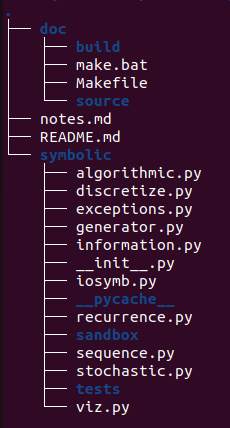
\includegraphics[width=4cm]{arborescence.png}
    \caption{Arborescence (de profondeur 2) du module scikits-symbolic}
    \label{fig5.1}
\end{figure}

\vspace{2ex}
On affiche ici seulement les principaux fichiers .py sans expliciter le contenu des autres répertoires. Toutefois, il est important de noter que le module est également composée de fichiers .rst dans les répertoires souce et build permettant la création de la documentation via Sphinx, que l'on détaillera plus tard, ainsi que d'autres fichiers sous-jacents permettant le fonctionnement du module scikits-symbolic. On va ici présenter seulement les différents fichiers sur lesquels j'ai apporté une contribution.

\vspace{2ex}
Le fichier central de scikits-symbolic est sequence.py où sont définis les différentes classes ainsi que leurs méthodes associées. Il y a 3 classes différentes, la classe State permet de définir un état. On peut créer un état, celui-ci représente et constitue le lien entre un entier et un symbole (qui peut-être une lettre d’un alphabet). 

\vspace{2ex}
La seconde classe est l’Alphabet. L’alphabet est une liste d’état, il peut être créé à partir d’une liste de States définis préalablement ou bien en donnant simplement le nombre de symboles que l’on souhaite dans notre alphabet. Cet objet  constitue une des deux bases indispensables à la définition d’une représentation symbolique. En effet, l’alphabet permet de conserver la représentation de la dynamique symbolique comme un vecteur de nombres entiers (facilement manipulable pour des calculs de la théorie de l’information) tout en ayant le lien visible avec la signification de chaque entiers de par leur association avec les symboles de l’alphabet. 

\vspace{2ex}
La dernière classe qui est au centre de nos intérêts et constitue la pièce centrale du scikit est donc l’objet Sequence qui permet de définir informatiquement une séquence symbolique. On voit donc que ces 3 classes sont imbriquées les unes dans les autres. La définition d’un objet séquence symbolique nécessite un vecteur qui est la séquence d’entier ainsi qu’un alphabet. Et la création d’un alphabet nécessite la définition des différents States qui le constituent.
De cette manière, la classe sequence permet d'avoir un objet informatique contenant toutes les propriétés et informations nécessaires pour correspondre au concept de séquence symbolique et donc à sa définition mathématique. 
Les méthodes implémentées pour la classe sequence permettent donc en autres d'obtenir la taille d'une séquence symbolique ainsi que la taille de son alphabet, de calculer son entropie de Shannon, etc. Il est également possible de créer une séquence symbolique à partir de deux séquences symboliques à condition qu'elles soient de même taille grpave à la fonction recode. Cela est possible pour deux séquences symboliques ayant des alphabets différents et même de taille différente. Cette fonction crée donc un nouvel alphabet qui prend en compte les symboles contenu dans les alphabets d'origine. Comme expliqué dans la partie 4.2.2, c'est une fonction que l'on a utilisé pour obtenir une séquence symbolique globale à partir de séquences symboliques représentées dans l'espace des phases de séries temporelles singulières des capteurs (projetés après une SVD). Cette séquence symbolique permet alors de rendre compte de la dynamique cérébrale globale.

\section{Fonctions}

Le reste du scikit est un ensemble de fonctions et de méthodes permettant de manipuler et de faire des opérations et des calculs au sens de la théorie de l’information sur des séquences symboliques que nous présentons ici :

\begin{enumerate}
    \item algorithmic : contient les différentes versions de l'estimateur du taux d'entropie de Lempel-Ziv;
    \item stochastic : permet le calcul des matrices de transition, matrices conditionnelles et d'influence de deux séquences symboliques qui représentent des processus stochastiques;
    \item information : permet le calcul de de différentes métriques issues de la théorie de l'information. Parmis celles-ci, on pourra citer l'information mutuelle de deux séquences symboliques ou plus, l'entropie de Shannon, etc;
    \item discretize : contient les fonctions permettant l'extraction de séquences symboliques à partir de séries temporelles
\end{enumerate}

\vspace{2ex}
Les fonctions du fichier discretize correspondent aux implémentations des méthodes de représentation symbolique explicitées dans la partie 4.2.

\section{Tests sur le scikits et documentation associée}

\vspace{2ex}
La convergence et les fondements théoriques des différents codes du module scikits-symbolic sur lesquels j'ai effectué les tests ont déjà été prouvés. Mon travail était donc de vérifier la correction des différents algorithmes. J'ai implémenté les tests directement sur le code, grâce au module Doctest qui permet d'écrire un test directement dans la définition de la fonction ou de la classe. On écrit les tests entre guillements, comme si l'on écrivait dans un document texte. En effet, le module Doctest permet d'écrire des prompts de commande que l'ordinateur va éxecuter lorsque qu'il va run le code. Comme on peut le voir en Figure \ref{fig5.3}, on écrit des commandes comme si les écrivait directement dans un shell Python avec ">>>" en amont pour indiquer une requête. Les lignes sans ">>>" correspondent à ce qu'est censé renvoyé l'ordinateur lors de la lecture des commandes, ici 0.6. On peut donc lui faire exécuter une suite de commandes qui utilisent les fonctions et les objets du module scikits-symbolic sur un exemple dont on connaît déjà le résultat. De cette manière, on vérifie que l'implémentation des scripts qui composent le module a été correctement effectuée et que l'algortithme produit les résultats attendus. C'est la vérification informatique de la correction de l'algorithme. Si la sortie est égale avec ce que l'ordinateur a calculé en suivant notre suite de commande, alors le test est concluant et aucun messages d'erreur ne s'affiche. Par contre, si le résultat obtenu est différent de ce qui est censé être trouvé, un message d'erreur s'affiche et cela permet de mettre en exergue un mauvais fonctionnement du code qui ne fait pas ce que l'on voudrait qu'il fasse (Figure \ref{fig5.3}).

\begin{figure}[!ht]
    \centering
    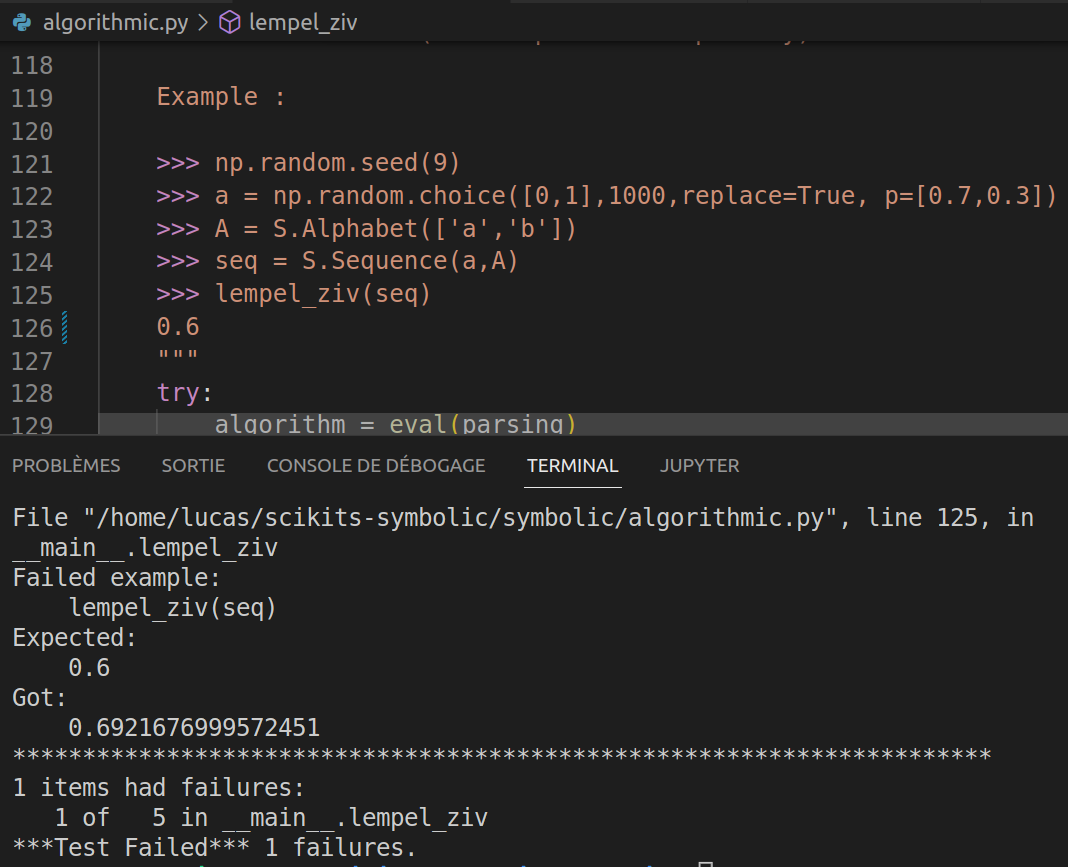
\includegraphics[width=13cm]{exemple_doctest.png}
    \caption{Exemple d'un test réalisé avec Doctest échoué. Expected représente ce que l'on a indiqué comme étant la sortie de notre ligne de commande "lempel-ziv(seq)", i.e., ce qu'est censé obtenir l'ordinateur lorsqu'il run le script en question. J'ai volontairement mis un résultat érroné pour pouvoir afficher le message d'erreur d'un test echoué. Got correspond au résultat effectivement obtenu par l'ordinateur lors de la lecture du script.}
    \label{fig5.3}
\end{figure}

\vspace{2ex}
Cette manière de tester en écrivant directement dans la définition d'une classe ou d'une fonction allait de paire avec la création d'une documentation pour le scikits-symbolic. En effet, le générateur de documentation Python Sphinx permet de générer facilement une documentation en prenant les informations contenues dans la définition d'une classe ou d'une fonction. Il suffit alors de décrire ce que fait notre code, de renseigner les différents paramètres avec une certaine typologie, d'écrire les test Doctest, tout cela au même endroit dans le code. Quelques manipulations des outils apportés par Sphinx nous permettent ensuite de générer un document pdf ou bien une page html en décidant de la structure. La documentation est consultable en deuxième partie de l'Annexe.
